\documentclass{esg8012pset}
\begin{preamble}
  \usepackage{amsmath}
  \usepackage{amssymb}
  \usepackage{enumerate}
  \usepackage{graphicx}
  \usepackage{hyperref}
  \providecommand{\uvec}[1]{{\hat{\bf{#1}}}}
  \usepackage{pgf,tikz}
  \usetikzlibrary{arrows}
  \makeatletter
  \newcommand{\interitemtext}[1]{%
    \begin{list}{}
     {\itemindent=0mm\labelsep=0mm
     \labelwidth=0mm\leftmargin=0mm
     \addtolength{\leftmargin}{-\@totalleftmargin}}
      \item #1
    \end{list}
  }
  \makeatother
  \renewcommand{\d}{\,d}
  \providecommand{\norm}[1]{\lVert#1\rVert}
\end{preamble}

\classname{Physics 8.012}
\semester{Fall 2010}
\problemsetnumber{4}
\date{October 1}
\makeatletter
\duedate{Friday, October 15}
\readingassignment{Kleppner and Kolenkow, \emph{An Introduction to Mechanics}, Chapter Three}

\begin{document}

\noindent Problems: Chapter 3: 1, 3, 4, 6, 7, 11, 12

\begin{problem}{K\&K 3.1}
  The density of a thin rod of length $l$ varies with distance $x$ from one end as $\lambda = \lambda_0 x^2 / l^2$.  Find the position of the center of mass.
\end{problem}
\begin{solution}
  The center of mass is the position $\displaystyle \frac{1}{m} \int \lambda x\d{x} = \frac{1}{\int_{0}^l \lambda_0 \frac{x^2}{l^2}\d{x}} \int_0^l \lambda_0 \frac{x^3}{l^2}\d{x} = \frac{1}{\lambda_0\frac{l^3}{3l^2}}\cdot\lambda_0\frac{l^4}{4l^2} = \frac{3}{l}\cdot \frac{l^2}{4} = \frac{3}{4}l$.
\end{solution}


\begin{problem}{K\&K 3.3}
  Suppose that a system consists of several bodies, and that the position of the center of mass of each body is known. Prove that the center of mass of the system can be found by treating each body as a particle concentrated at its center of mass.
\end{problem}
\begin{solution}
  We treat the bodies as composed of distinct particles, and allow infinite sums and infinitesimal masses.  Suppose we have bodies of masses $m_i$ with centers of mass $\vec x_i$, for $i\in I$.  Suppose that each body $i$ consists of particles with masses $m_{i, j}$ and positions $\vec x_{i, j}$ for $j\in J_i$.  Then the center of mass of the system is 
  $$\frac{\displaystyle \sum_{i\in I} \sum_{j\in J} m_{i, j}\vec x_{i, j}}{\displaystyle \sum_{i\in I} \sum_{j\in J} m_{i, j}}$$
  By assumption, $\sum_{j\in J} m_{i, j} = m_i$, the total mass of object $i$, and $\left(\sum_{j\in J} m_{i, j}\vec x_{i, j}\right) / \left(\sum_{j\in J} m_{i, j}\right) = \vec x_i$, the center of mass of object $i$.  Then, by simplification, the center of mass of the system is 
  $$\frac{\displaystyle \sum_{i\in I} m_i \vec x_i}{\displaystyle \sum_{i\in I} m_i}$$
  Since this is the result of the center of mass calculation under the assumption that each body is a point mass, at its center of mass, the center of mass of the system can be found by treating each body as a particle concentrated at its center of mass.
\end{solution}



\begin{problem}{K\&K 3.4: Exploding Projectile}
  An instrument-carrying projectile of mass $m_1$ accidentally explodes at the top of its trajectory. The horizontal distance between launch point and the explosion is $x_0$.  The projectile breaks into two pieces which fly apart horizontally. The larger piece, $m_3$, has three times the mass of the smaller piece, $m_2$. To the surprise of the scientist in charge, the smaller piece returns to earth at the launching station. Neglect air resistance and effects due to the earth's curvature.
  \begin{center}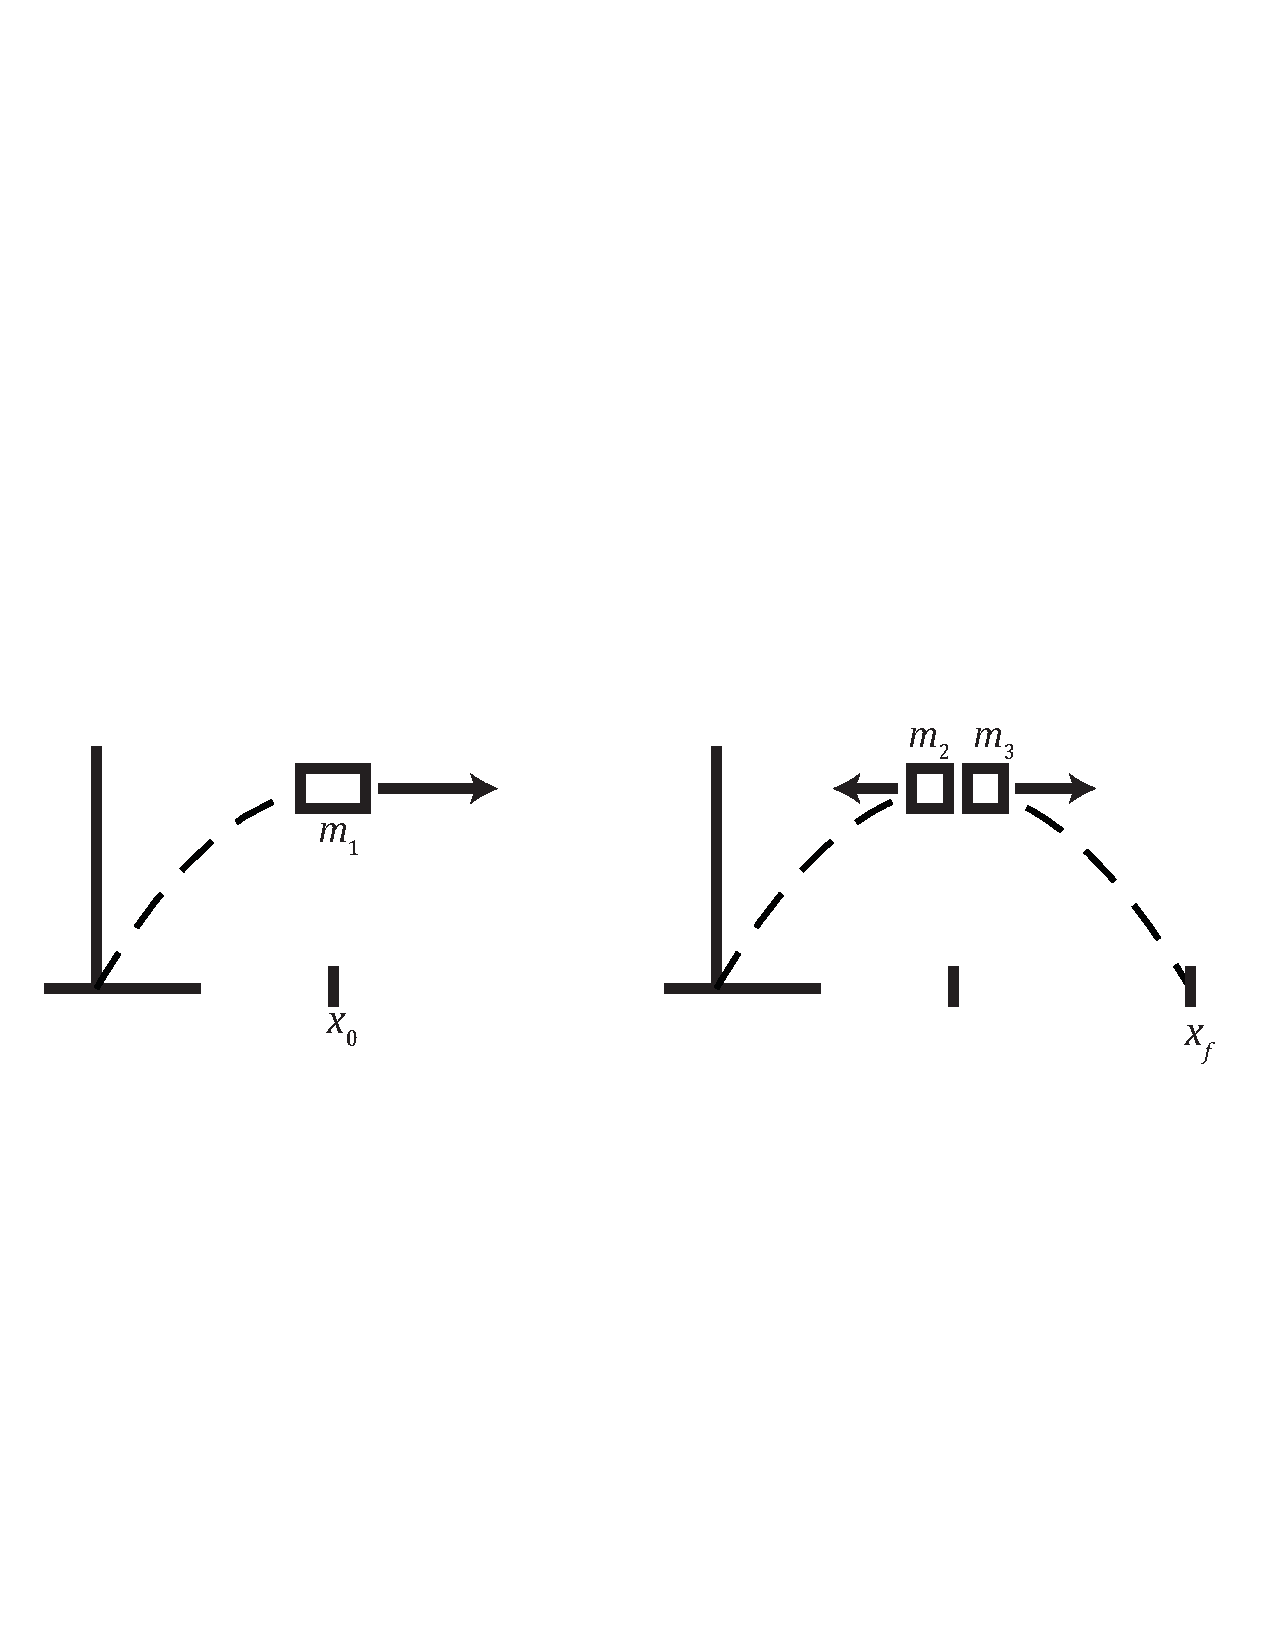
\includegraphics[width=0.5\textwidth]{ps_04_1}\end{center}
%\begin{enumerate}[a)]
%  \item What is the velocity of the projectile at the top of its flight just before the collision?
%  \item What is the velocity of the smaller piece just after the collision?
%  \item What is the velocity of the larger piece just after the collision?
%  \item 
  How far away, $x_f$, from the original launching point does the larger piece land?
%\end{enumerate}
\end{problem}
\begin{solution}
  Let $v$ be the velocity of the projectile just before the explosion.  Since the smaller piece returns to the launch site, $v_2 = -v$.  Then $v t = x_0$, and $m_1 v = -v m_2 + v_3 m_3$.  So $\frac{m_1+m_2}{m_3} v = v_3$.  Then $x_f - x_0 = v_3 t = \frac{m_1+m_2}{m_3}\cdot \frac{x_0}{t} \cdot t = \frac{m_1+m_2}{m_3}x_0$.  Since $m_3 = 3m_2$, and $4m_2 = m_1$, $x_f = \frac{5m_2}{3m_2}x_0 = \frac{5}{3}x_0$.
\end{solution}




\begin{problem}{K\&K 3.6}
  A light plane weighing 2500 lb makes an emergency landing on a short runway. With its engine off, it lands on the runway at a speed of 120 ft / sec. A hook on the plane snags a cable attached to a 250 lb sandbag and drags the sandbag along. If the coefficient of friction between the sandbag and the runway is $\mu_k = 0.4$, and if the plane's brakes give an additional retarding force of magnitude 300 lb, how far does the plane go before it comes to a stop?
\end{problem}
\begin{solution}
  $v_0 = 120$ ft / sec, $\dot v = \frac{-250\text{ lb}(0.4)}{2500\text{ lb} / g} - \frac{300\text{ lb}}{2500\text{ lb} / g} = -\frac{4}{25} g \approx -5.1478\text{ ft / s}^2$.  Then $v = 120\text{ ft / sec} -\frac{4}{25} g t$.  Then $v = 0$ at $t \approx 23.3$ s.  Then $\Delta x = 120\text{ ft / sec} t - \frac{2}{25} g t^2 \approx 1399$ ft.


  \noindent {\bf Correction:} $\frac{(2750\text{ lbs})(v_0) - (2500\text{ lbs})(120\text{ ft / s})}{\Delta t} = \mu_k (2750\text{ lbs})$, so $\frac{(1100\text{ lbs})(\Delta t) + (300000\text{ lbs ft / s})}{2750\text{ lbs}} = v_0$.  As $\Delta t \longrightarrow 0$, $v_0 = \frac{1200}{11}\text{ ft / s}$.  FIX Then $\dot v = \frac{-250\text{ lb}(0.4)}{2750\text{ lb} / g} - \frac{300\text{ lb}}{2750\text{ lb} / g} = -\frac{4}{25} g \approx -5.1478\text{ ft / s}^2$.  Then $v = 120\text{ ft / sec} -\frac{4}{25} g t$.  Then $v = 0$ at $t \approx 23.3$ s.  Then $\Delta x = 120\text{ ft / sec} t - \frac{2}{25} g t^2 \approx 1399$ ft.
\end{solution}



\begin{problem}{K\&K 3.7}
  A system is composed of two blocks 1 and 2 of masses $m_1$ and $m_2$ respectively that are connected by a massless spring with spring constant $k$. The blocks slide on a frictionless plane. The unstretched length of the spring is $l$. Initially the block 2 is held so that the spring is compresses to a length $l / 2$ and block 1 is pushed up against a wall. At $t = 0$ block 2 is released. Find the motion of the center of mass of the system as a function of time.
\end{problem}
\begin{solution}
  Let $x = 0$ be the position of block 2 when the spring is uncompressed.  Then the initial position of block 2, $x_{2,0} = -l/2$.  Until the spring is fully uncompressed, the first block is stationary, and the force on the second block is $F = -kx$.  Then $\frac{\d^2 x}{\d t^2} = -\frac{k}{m_2}x$.  Solutions to this equation are $A\cos(\omega t) + B\sin(\omega t)$.  Then $\omega = \sqrt{\frac{k}{m_2}}$.  At time $t = 0$, $x = -l/2$, so $A = -l/2$, so $x = -\frac{l}{2}\cos\left(\sqrt{\frac{k}{m_2}} t\right) + B\sin\left(\sqrt{\frac{k}{m_2}}t\right)$, and $v = 0$, so $B = 0$.  Then $x(t) = -\frac{l}{2}\cos\left(\sqrt{\frac{k}{m_2}} t\right)$.

  At time $t = t_1$, the spring is fully uncompressed, and $x = 0$, so $\cos\left(\sqrt{\frac{k}{m_2}} t_1 \right) = 0$.  Then $t_1 = \frac{\pi}{2}\cdot \sqrt{\frac{m_2}{k}}$.  At this point in time, $\dot x(t_1) = \frac{l}{2}\sqrt{\frac{k}{m_2}}\sin\frac{\pi}{2} = \frac{l}{2}\sqrt{\frac{k}{m_2}}$.  The momentum of the system at this point in time, is $\frac{l\sqrt{k m_2}}{2}$.  Since there is no external force on the system after this point in time, $(m_1 + m_2)v_{\text{center of mass}} = \frac{l\sqrt{k m_2}}{2}$.  Thus, $$v_{\text{center of mass}} = \begin{cases} \frac{l\sqrt{k m_2}\sin\left(\sqrt{\frac{k}{m_2}} t\right)}{2(m_1 + m_2)} & t < \frac{\pi}{2}\sqrt{\frac{m_2}{k}} \\ \frac{l\sqrt{k m_2}}{2(m_1 + m_2)} & t \geq \frac{\pi}{2}\sqrt{\frac{m_2}{k}} \end{cases}$$
\end{solution}


\begin{problem}{K\&K 3.11}
  Material is blown into cart A from cart B at a rate of $b$ kilograms per second. The material leaves the chute vertically downward, so that it has the same horizontal velocity, $u$ as cart B. At the moment of interest, cart A has mass $m_A$ and velocity $v$.
  \begin{center}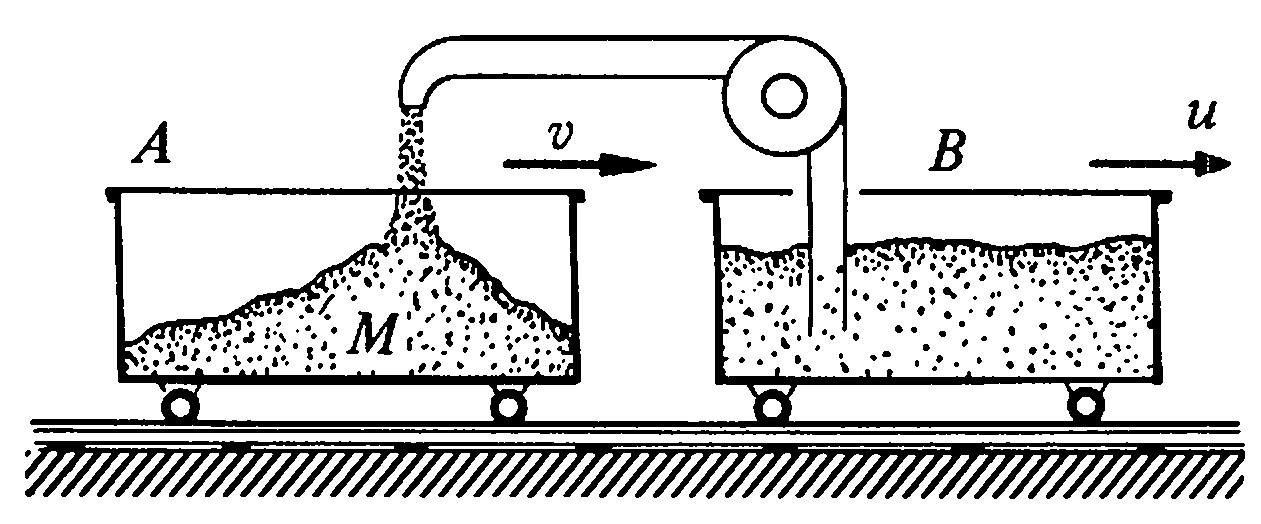
\includegraphics[width=0.5\textwidth]{ps_04_2}\end{center}
  \begin{enumerate}
    \item Define the objects that will constitute your system.
    \item Based on momentum diagrams, derive a differential equation for the velocity $v$.
    \item In particular find an expression for the rate of change of velocity, the instantaneous acceleration, $d v / d t$.
    \item Integrate this equation to find the velocity has a function of time.
  \end{enumerate}
\end{problem}
\begin{solution}
  \begin{enumerate}
    \item The system consists of cart $A$, and the material in it.
    \item $m_A v + \Delta m_A u = (m_A + \Delta m_A) (v + \Delta v)$, so $\Delta m_A u = m_A \Delta v + \Delta m_A v + \Delta m_A \Delta v$.  Then $u \frac{\Delta m_A}{\Delta t} = m_A\frac{\Delta v}{\Delta t} + v\frac{\Delta m_A}{\Delta t} + \Delta m_A \frac{\Delta v}{\Delta t}$.  Taking the limit as $\Delta t$ goes to 0, $u\frac{\d m_A}{\d t} = m_A \frac{\d v}{\d t} + v\frac{\d m_A}{\d t}$.  Then $ub = m_A \frac{\d v}{\d t} + vb$, so $v = u - \frac{m_A}{b}\frac{\d v}{\d t}$.
    \item $\frac{\d v}{\d t} = \frac{b}{m_A}(u - v)$
    \item $\frac{\d v}{u - v} = \frac{b\d t}{m_{A, 0} + bt}$, so $\int \frac{\d v}{u - v} = \int \frac{b\d t}{m_{A, 0} + bt}$, so $-\ln(u - v) = \int\frac{\d t}{\frac{m_{A,0}}{b} + t} = \ln\left(\frac{m_{A,0}}{b} + t\right) + C_1 = \ln(m_{A,0} + b t) + C_2$.  Then, $\frac{1}{u - v} = C_3 (m_{A,0} + bt)$, so $v(t) = u - \frac{C_4}{m_{A,0} + bt} = \frac{b t u + C_5}{m_{A, 0} + b t}$.  $m_{A, 0} = m_A$.  At time $t = 0$, $v(0) = v_0 = \frac{C_5}{m_A}$, so $C_5 = m_A v_0$.  Then $v(t) = \frac{b t u + m_A v_0}{m_A + b t}$. \par
    Alternatively: Evaluate $m_A v + \Delta m_A u = (m_A + \Delta m_A) (v + \Delta v)$ at time $t$; $v = v_0$, $v + \Delta v = v(t)$, and $\Delta m_A = b t$.  Then, $m_A v_0 + b t u = (m_A + b t)v(t)$, so $v(t) = \frac{b t u + m_A v_0}{m_A + b t}$.
  \end{enumerate}
\end{solution}



\begin{problem}{K\&K 3.12}
  A sand-spraying locomotive sprays sand horizontally into a freight car. The locomotive and freight car are not attached. The engineer in the locomotive maintains his speed so that the distance to the freight car is constant. The sand is transferred at a rate $d m / d t = 10$ kg/s with a velocity $u = 5$ m/s relative to the locomotive. The car starts from rest with an initial mass of 2000 kg. Find its speed after 100 s.
  \begin{center}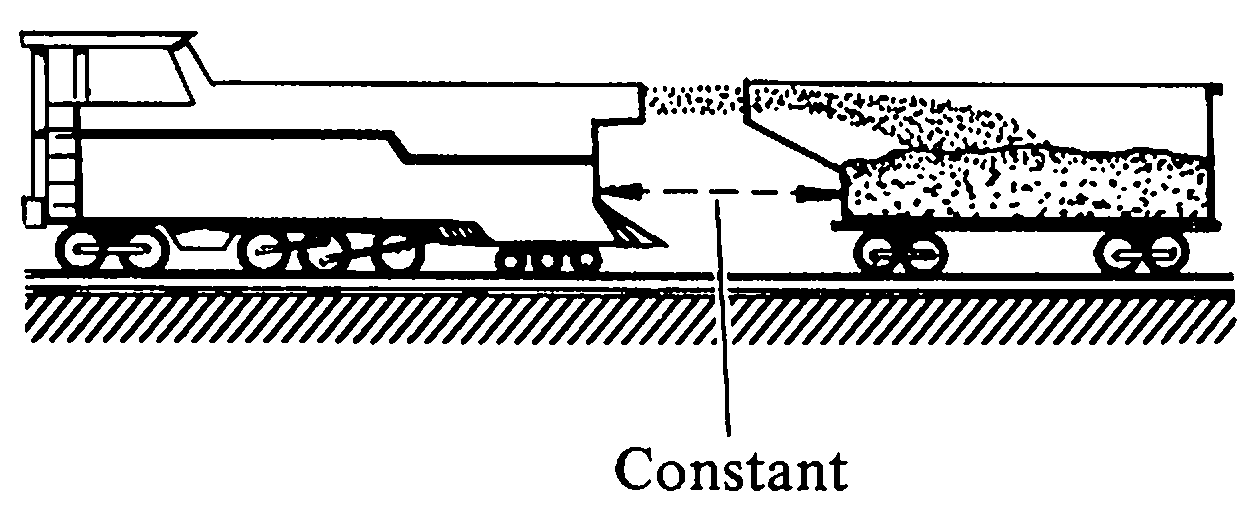
\includegraphics[width=0.5\textwidth]{ps_04_3}\end{center}
\end{problem}
\begin{solution}
  \begin{align*}
   m v + \Delta m (u + v) & = (m + \Delta m) (v + \Delta v) \\
   (u + v)\Delta m & \approx v\Delta m + m\Delta v \\
   u\frac{\d m}{\d t} & = m\frac{\d v}{\d t} \\
   u\frac{\d m}{m} & = \d v \\
   \int_{m_0}^{m} u\frac{\d m}{m} & = \int_{0}^{v} \d v \\
   u(\ln m - \ln m_0) & = v \\
   v & = u\ln\frac{m}{m_0} \\
   v(t) & = (5\text{ m / s})\ln\frac{2000\text{ kg} + (10\text{ kg / s})t}{2000\text{ kg}} \\
   v(100\text{ s}) %& = (5\text{ m / s})\ln\frac{3}{2} \\
    & = 5\ln(3 / 2)\text{ m / s}
  % m\frac{\d v}{\d t} & = u\left(\frac{\d m}{\d t}\right) \\
  % \d v & = u\left(\frac{\d m}{\d t}\right)\frac{\d t}{m} \\
  % \d v & = u\left(\frac{\d m}{\d t}\right)\frac{\d t}{m_0 + \left(\frac{\d m}{\d t}\right)t} \\
  % \int \d v & = u\left(\frac{\d m}{\d t}\right)\int \frac{\d t}{m_0 + \left(\frac{\d m}{\d t}\right)t} \\
  % v & = u\left(\frac{\d m}{\d t}\right)\ln\left(m_0 + \left(\frac{\d m}{\d t}\right)t\right) + C_1 \\
  % \intertext{Since $v(0) = 0$,}
  % 0 & = u\left(\frac{\d m}{\d t}\right)\ln\left(m_0\right) + C_1 \\
  % C_1 & = -u\left(\frac{\d m}{\d t}\right)\ln\left(m_0\right) \\
  % v & = u\left(\frac{\d m}{\d t}\right)\ln\left(m_0 + \left(\frac{\d m}{\d t}\right)t\right) - u\left(\frac{\d m}{\d t}\right)\ln m_0 \\
  % v(t) & = (5\text{ m / s})(10\text{ kg / s})\ln\left(2000\text{ kg} + (10\text{ kg / s})t\right) - (5\text{ m / s})(10\text{ kg / s})\ln(2000\text{ kg})\\
  %  & = 50\text{ N}\ln(2000\text{ kg} + (10\text{ kg / s})t) - 50\text{ N}\ln(2000\text{ kg})
  \end{align*}
  %Since $v(0) = 0$, $C_1 = -u\ln m_0 = -(5\text{ m / s})\ln(
\end{solution}
\end{document}
